% !TeX TS-program = xelatex

\documentclass[aspectratio=169]{beamer}

\usepackage{xltxtra}
\usepackage{csquotes}
\usepackage[main=russian,english]{babel}
\defaultfontfeatures{Mapping=tex-text}

% Chinese support
\usepackage{xeCJK}

% tikz
\usepackage{tikz}
\usetikzlibrary{positioning,shapes}

\usepackage{ulem}

\usetheme{sm2022}

% add bib -file
\addbibresource{golang-map-internals-fob.bib}

\title{Устройство map в Golang ~\\// Failover bar}
\author{Филипп Кулин}
\date{20 июня 2022}

\begin{document}

\begin{frame}
\titlepage
\end{frame}

\begin{frame}{Preface}
        \begin{itemize}
                \item Презентация сделана на \LaTeX
                \item Презентация размещена на github\\
                \textcolor{blue}{\href{https://github.com/schors/gmi2022-fob}{https://github.com/schors/gmi2022-fob}}
                \item<2-> О, Великий Один, я торопился
        \end{itemize}
\end{frame}

\begin{frame}
        \center \huge map в Golang \\ --- \\ хэш таблица
\end{frame}

\begin{frame}{Хэш таблица}
        Таблица
        \begin{itemize}
                \item Ключу \texttt{key} сопостовляется значение \texttt{value}
                \item Операции:
                \begin{itemize}
                        \item Вставки
                        \item Поиска
                        \item Удаления
                \end{itemize}
        \end{itemize}
        ~\\
        Хэш таблица
        \begin{itemize}
                \item Поиск по хэшу ключа
                \begin{itemize}
                        \item Константное или линейное время поиска \\
                        \textit{\small O(1) или O(n)}
                \end{itemize}
        \end{itemize}
\end{frame}

\begin{frame}{Что такое "хэш"}
        \begin{itemize}
                \item Результат выполнения хэш функции
                \begin{itemize}
                        \item Преобразование данных произвольной длины в данные установленной длины
                \end{itemize}
                \item Изменение данных приводит к изменению хэша
                \item Разные данные могут иметь один хэш --- коллизии
                \begin{itemize}
                        \item Вероятность коллизий --- мера качества хэш-функции
                \end{itemize}
        \end{itemize}
\end{frame}


\begin{frame}[fragile]{Тип данных map}
        Тип \texttt{map[KeyType]ValueType}
        \begin{itemize}
                \item KeyType: логические (bool), числовые, строки, указатели, каналы, интерфейсы, структуры и массивы\\
                \textit{\small те, что могут сравниваться (==)}
                \item \textbf{НЕ могут} быть ключами: срезы, map, функции
        \end{itemize}
        ~\\
        map --- ссылочный тип, как срез и указатель\\
        ~\\
        \begin{columns}[t,onlytextwidth]
                \begin{column}{0.48\textwidth}
                        \begin{lstlisting}
var m map[string]int\end{lstlisting}
                \end{column}
        \end{columns}
\end{frame}

\begin{frame}
        \center \huge Залезем под капот
\end{frame}

\begin{frame}[fragile]{Что иль кто есть map'а?}
        // \textcolor{blue}{\href{https://go.dev/src/runtime/map.go}{https://go.dev/src/runtime/map.go}}
        ~\\
        Функция создания возвращает указатель на структуру
        \begin{lstlisting}
// makemap implements a Go map creation make(map[k]v, hint)

func makemap(t *maptype, hint int, h *hmap) *hmap\end{lstlisting}
        ~\\
        Компилятор заменяет конструкции функциями
        \begin{lstlisting}
v := m["ключ"]          // → runtime.mapaccess1(m, "ключ")

v, ok := m["ключ"]      // → runtime.mapaccess2(m, "ключ")

m["ключ"] = "значение"  // → runtime.mapassign(m, "ключ")

delete(m, "ключ")       // → runtime.mapdelete(m, "ключ")\end{lstlisting}
\end{frame}

\begin{frame}{Конкурентная работа с map}
        \begin{itemize}
                \item Всегда \texttt{sync.(RW)Lock} при конкурентной записи
                \begin{itemize}
                        \item Все операции состоят из набора функций
                        \begin{itemize}
                                \item Планирование в прологах функцмй
                        \end{itemize}
                \end{itemize}
                \item Только конкурентное чтение блокировки не требует
        \end{itemize}
\end{frame}

\begin{frame}[fragile]{Заголовок map'ы}
        \begin{lstlisting}
type hmap struct {
    count     int     // # кол-во элементов, len()
    flags     uint8
    B         uint8  // log_2 числа корзин, размер
    noverflow uint16 // примерное кол-во допкорзин
    hash0     uint32 // hash seed

    buckets    unsafe.Pointer // массив корзин
    oldbuckets unsafe.Pointer // устаревшие корзины (при росте)
    nevacuate  uintptr        // прогресс эвакуации

    extra *mapextra // дополнительные данные
}\end{lstlisting}
\end{frame}

\begin{frame}
        \center \huge Папа, ты с кем сейчас разговаривал?
\end{frame}

\begin{frame}{Корзины}
        \begin{columns}[t,onlytextwidth]
                \begin{column}{0.50\textwidth}
                        \begin{itemize}
                                \item Данные хранятся в корзинах
                                \item В корзине 8 элементов
                                \item \texttt{bucketSize * \\(1+maxKeySize+maxValSize)\\+ ptrSize}\\
                                // \textcolor{blue}{\href{https://go.dev/src/reflect/type.go}{https://go.dev/src/reflect/type.go}}
                                \item TOP[N] --- первый байт хэша ключа
                                \begin{itemize}
                                        \item $<$ 5: флаги (пусто, конец, эвакуация)
                                        \item реальные данные: приводится к $>=$ 5
                                \end{itemize}
                        \end{itemize}
                \end{column}
                \begin{column}{0.48\textwidth}
                        \begin{figure}
                                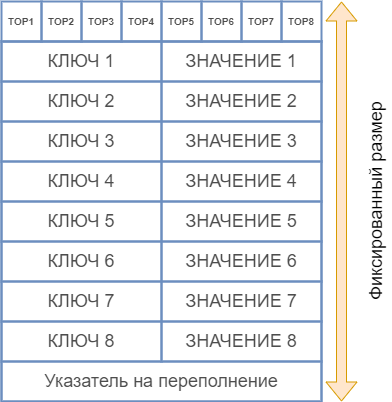
\includegraphics[width=0.85\textwidth]{img/bucketsize.png} \\
                        \end{figure}
                \end{column}
        \end{columns}
\end{frame}

\begin{frame}{Поиск в корзине}
        \begin{columns}[t,onlytextwidth]
                \begin{column}{0.50\textwidth}
                        \begin{itemize}
                                \item TOP --- первый байт хэша искомого ключа
                                \item TOP[N] --- первый байт хэша записанного ключа
                                \item TOP[N] == 0: поиск останавливается
                                \item TOP == TOP[N]: сравниваются значения ключей
                                \item Ключи не равны: ищем дальше
                        \end{itemize}
                \end{column}
                \begin{column}{0.48\textwidth}
                        \begin{figure}
                                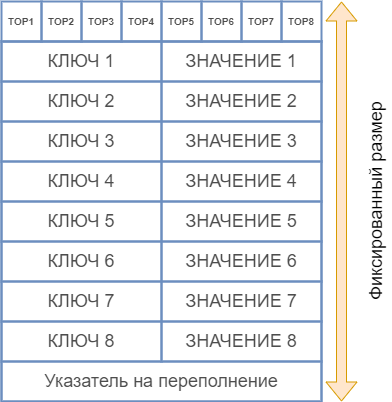
\includegraphics[width=0.85\textwidth]{img/bucketsize.png} \\
                        \end{figure}
                \end{column}
        \end{columns}
\end{frame}

\begin{frame}{Организация корзин. Адресация}
        Размер map'ы hash.B
        \begin{itemize}
                \item $2^{hash.B}$ --- количество корзин
                \item hash.B --- маска значимых битов хэша ключа \\
                \item Значимые биты --- индекс в массиве корзин
        \end{itemize}
\end{frame}

\begin{frame}[label=buckets]{Устройство map}
        \begin{figure}
                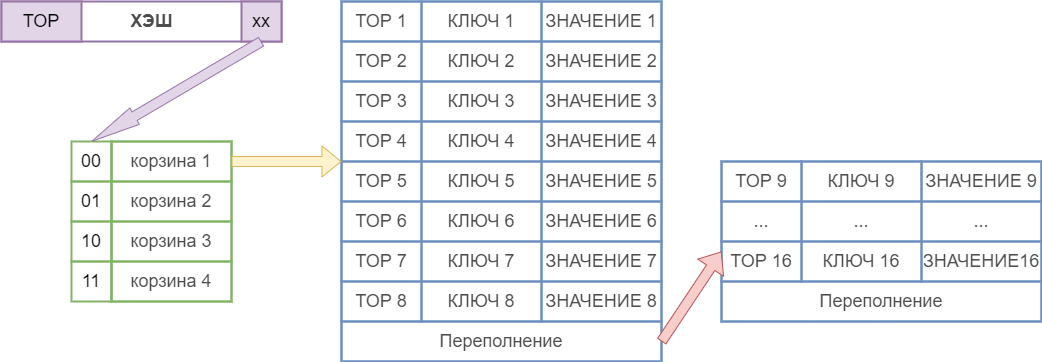
\includegraphics[width=0.85\textwidth]{img/buckets.png} \\
        \end{figure}
        \begin{itemize}
                \item Количество корзин == маска хэша
                \item Внутри корзины поиск перебором
        \end{itemize}
\end{frame}

\begin{frame}{Выбор хэш-функции}
        Условия
        \begin{itemize}
               \item Быстрая
               \item Низкая вероятность коллизий
               \item Хороший разброс (для уменьшения переполнений)
               \item Каждая таблица имеет свою уникальную "затравку" \\
               \textit{\small хэш одних и тех же данных будет разным у разных экземпляров таблиц}
        \end{itemize}
        ~\\
        Реализация
        \begin{itemize}
                \item Отдельные функции для ключей размера 32,64 бита и строк
                \item Генерируемые компилятором функции для остальных
                \item Меняются от версии к версии и на разных платформах\\
                \textit{\small например на amd64 пытается использовать AES процессора}
        \end{itemize}
\end{frame}

\againframe{buckets}

\begin{frame}{Рост map}
        Условия
        \begin{itemize}
                \item Или среднее количество значений в корзине \textbf{6.5}
                \item Или слишком много переполнений (формула)
        \end{itemize}
        ~\\
        Что происходит
        \begin{itemize}
                \item Создаётся в два раза больше корзин
                \begin{itemize}
                        \item Если корзин 16 и больше, резервируется место для переполнений
                \end{itemize}
                \item На записи и удалении данные мигрируют (эвакуируются)
        \end{itemize}
        ~\\
        \textbf{Таблицы только растут}
\end{frame}

\begin{frame}{Особые случаи}
        \begin{itemize}
                \item Если размер ключа или значение больше 128 байт, они размещаются отдельно (аллокация)
                \item Маленькая таблица до 8 значений будет размещена в стеке
                \item Пустая структура \texttt{struct{}} имеет нулевой размер
        \end{itemize}
\end{frame}

\begin{frame}{Всё --- тлен}
        \begin{itemize}
                \item Алгоритмы внутренних механизмов все время меняются
                \item 4 года назад все было не так
                \item Через год --- всё будет иначе
        \end{itemize}
\end{frame}

\begin{frame}
        \center \huge Вопросы?
\end{frame}

\nocite{*}
\setbeamertemplate{frametitle continuation}{}
\begin{frame}[t]{Ссылки}
\printbibliography
\end{frame}

\end{document}


